\documentclass{article}
\usepackage{graphicx}

\title{The Youtube Math Channels}
\author{Michael Yang}

\begin{document}

\maketitle
It's no secret that there is some great educational math content on the internet -- however, one area that often goes a bit overlooked is YouTube! Here are a few quick introductions to some of the main math YouTubers. 
\begin{center}

\includegraphics[scale=0.35]{images/youtube.2022.12.png}
\end{center}
The channel Numberphile, run by videographer Brady Haran, is perhaps the oldest well-known math channel still producing videos. Originally with videos focusing exclusively on one number and documenting several interesting facts about it, Numberphile has now broadened its scope to more general mathematical topics. For each video, Brady chooses a well-known mathematician to interview about a topic of their choice. Amazing math is then presented on Numberphile's classic brown paper, giving it a familial aura while also exploring some genuinely deep and fascinating topics. Additionally, videos are released quite frequently (often with just a few weeks between them!), and the interviewed mathematicians come from a variety of diverse cultures and backgrounds. Some highlights of Numberphile include Neil Sloane talking about incredible sequences, Hannah Fry on the mathematics of love, and Matt Parker with the Parker Square. Speaking of which... 
\begin{center}

\includegraphics[scale=0.35]{images/numberphile.png}
\end{center}
Of famed mathematical hilarity, the channel Stand-Up Maths is becoming more and more well-known. Run by mathematician Matt Parker, the channel aims to make math easy and fun to learn through the unlikely medium of stand-up comedy. In each video, Matt tackles what seems at first like a horribly difficult math problem with a mix of intriguing computer visuals, deep research papers, silly physical props, and his trademark enthusiasm. Known for "giving things a go," Matt is more than happy to post his (occasionally embarrassing!) attempts at tasks such as proving unsolved conjectures and measuring the radius of the Earth on the internet. What's never compromised, though, is the math(s): Matt is always sure to make his arguments airtight and is always willing to point out one of his past mistakes. 

Perhaps viewed as the gold standard of production quality, mathematician Grant Sanderson's channel 3blue1brown is a gold mine for eloquent explainers on some seriously intriguing math. Grant's education is no joke -- he graduated with a math degree from Stanford -- but his clear and intuitive explanation style has won over the hearts of many a math enthusiast. 
\begin{center}
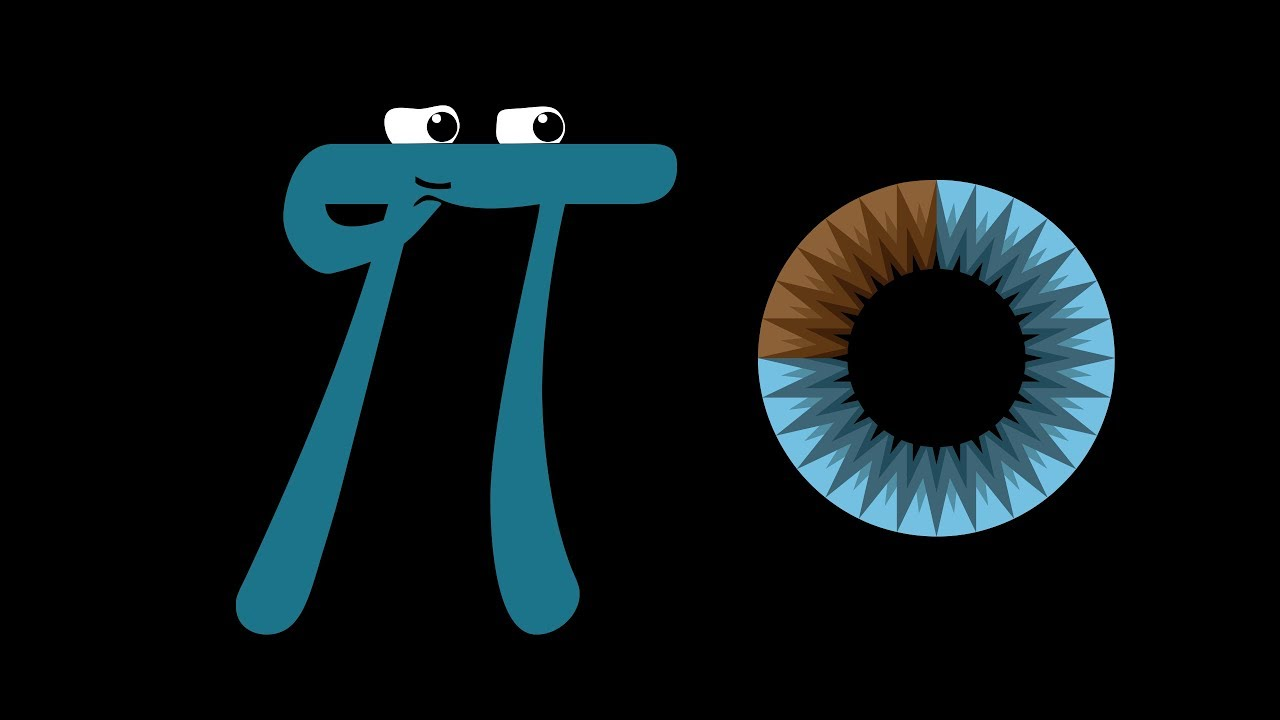
\includegraphics[scale=0.125]{Magazines/img/Vol3/3b1b.jpg}
\end{center}
With an emphasis on building intuition over rote computation, each 3blue1brown video strives to emphasize the visual beauty of mathematics. Perhaps unsurprisingly, the quality is top-notch: with fluid animations put together with meticulous care, Grant has cultivated a unique style and online presence. His video series on Calculus and Linear Algebra, in particular, have served as helpful building blocks for many future learners; his "Lockdown Math" livestreams, done in the middle of the pandemic for a high-school audience, has also garnered critical acclaim. 

Of course, there are many more excellent math-related YouTube channels out there (Vihart and Veritasium, anyone?) as well, and this is by no means an exhaustive list. And while YouTube is of course not an exhaustive math repository, it can be a useful resource for finding both quirky mathematical facts or deep proofs to some of the hardest theorems of our day.
\end{document}